\documentclass[a4paper]{article}
\usepackage{fontspec}
\usepackage{fontenc}
\usepackage{extarrows}
\usepackage{chemfig}
\usepackage[version=4]{mhchem}
\usepackage{mwe}
\usepackage{amsmath}
\usepackage{fancyhdr}
\usepackage{graphicx}
\usepackage{color}
\usepackage{amssymb}
\usepackage{siunitx}
\usepackage{bigfoot}
\usepackage{fancyvrb}
\usepackage{expl3}
\usepackage{calc}
\usepackage{geometry}
\geometry{left=2.5cm,right=2.5cm,top=2cm,bottom=3cm}
\setmainfont{Hiragino Sans GB}

\title{化学实验}
\author{胡译文}
\date{\today}

\makeatletter
\newcommand{\figcaption}{\def@captype{figure}\caption}
\newcommand{\tabcaption}{\def@captype{table}\caption}
\makeatother

\XeTeXlinebreaklocale "zh"
\XeTeXlinebreakskip = 0pt plus 1pt

\usepackage{hyperref}
\renewcommand\contentsname{目录}

\begin{document}
	\maketitle
	\begin{center}
		若有bug请到{\color{red}\href{https://github.com/huyiwen/Chem}{github}}上提Issue。\\
		技术有限所有方程式的等号都用箭头代替了。
	\end{center}
	\renewcommand\contentsname{目录}
	\tableofcontents
	
	
	\clearpage
	\section{基本仪器}
	
	
	\subsection{容器}
	\begin{itemize}
		\item 直接加热:
			\begin{itemize}
			\item 试管:倾斜$\ang{45}$,加热时液体不超过$1/3$
			\item 坩锅:在泥三角上加热,用坩埚钳夹取
			\item 蒸发皿:玻璃棒搅拌,用 坩埚钳夹取
			\end{itemize}
		\item 隔网加热:
			\begin{itemize}
			\item 烧杯
			\item 烧瓶:圆底烧瓶(承装液体不超过2/3)、蒸馏烧瓶(有支管、用于蒸馏制气体)、平底烧瓶
			\item 锥形瓶
			\end{itemize}
		\item 不能加热:集气瓶、表面皿
	\end{itemize}
	
	
	\subsection{量器}
	\begin{itemize}
		\item 粗量仪器:托盘天平、量筒、温度计
		\item 精量仪器:容量瓶、滴定管
	\end{itemize}
	
	\subsubsection{温度计}
	\paragraph{测反应混合物的温度}
	这种类型的实验需要测出反应混合物的准确温度,因此,应将温度计插入混合物中间。
	\begin{itemize}
		\item 测物质溶解度
		\item 实验室制乙烯
	\end{itemize}
	\paragraph{测蒸气的温度}
	这种类型的实验,多用于测量物质的沸点,由于液体在沸腾时,液体和蒸气的温度相同,所以只要测蒸气的温度。
	\begin{itemize}
		\item 实验室蒸馏石油
		\item 测定乙醇的沸点
	\end{itemize}
	\paragraph{测水浴温度}
	这种类型的实验,往往只要使反应物的温度保持相对稳定,所以利用水浴加热,温度计则插入水浴中。
	\begin{itemize}
		\item 温度对反应速率影响的反应
		\item 苯的硝化反应
	\end{itemize}
	
	\subsubsection{容量瓶}
	\paragraph{使用方法}
	\begin{enumerate}
		\item 检漏:加水,塞好瓶塞,倒立,瓶塞周围无水漏出,将瓶正立并将瓶塞旋转$\ang{180}$后塞紧,再倒立,无水漏出
		\item 计算
		\item 称量(天平、药匙)或量取(量筒)
		\item 溶解或稀释: 在烧杯中加适量水溶解或稀释,玻璃棒搅拌,冷却。
		\item 移液:玻璃棒引流
		\item 洗涤:洗涤烧杯,洗涤液也转移到容量瓶内, 次。
		\item 定容:先玻璃棒引流加水至刻度线下$1~2cm$处,然后用胶头滴管滴加至平视凹液面最低处与刻度线相平
		\item 摇匀:左手顶在瓶塞,右手五指轻托平底,反复颠倒上下摇匀
	\end{enumerate}
	\paragraph{注意事项}
	\begin{itemize}
		\item 不能在容量瓶里进行溶质的溶解,应将溶质在烧杯中溶解、冷却后转移
		\item 溶液不能超过容量瓶的标线,一旦超过,必须重新进行配制
		\item 容量瓶不能进行加热
		\item 选用时需要标明规格($1/2.5/5\times 10^n mL$)
	\end{itemize}
	
	\subsubsection{滴定管}
	\begin{itemize}
		\item 酸式滴定管(玻璃旋钮):不能用于碱性物质
		\item 碱式滴定管(橡胶管):不能用于强氧化性物质和有机溶剂
	\end{itemize}
	
	
	\subsection{分离仪器}
	\begin{itemize}
		\item 固液分离:普通漏斗
		\item 液液分离:分液漏斗
		\item 气气分离:洗气瓶、干燥管
	\end{itemize}
	
	\subsubsection{干燥管}
	\paragraph{种类}
	球形干燥管(固体干燥剂)、U形干燥管(液体或固体干燥剂)
	\paragraph{常见干燥剂}
	\begin{itemize}
		\item 浓\ce{H2SO4}:酸性干燥剂
		\item \ce{P2O5}固体:酸性干燥剂
		\item 碱石灰:碱性干燥剂
		\item 无水\ce{CaCl2}:中性干燥剂,不能干燥\ce{NH3}
		\item 无水\ce{CuSO4}:中性干燥剂,万能干燥剂
		\item 无水\ce{MgSO4}:中性干燥剂、有机干燥剂
		\item 无水\ce{Na2SO4}:中性干燥剂、有机干燥剂
	\end{itemize}
	
	
	\subsection{热源}
	\begin{itemize}
		\item 酒精灯、酒精喷灯
	\end{itemize}
	
	
	\subsection{其他}
	\begin{itemize}
		\item 玻璃棒、胶头滴管、冷凝管、水槽、铁架台
	\end{itemize}
	
	\subsubsection{冷凝管}
	\begin{itemize}
		\item 直形冷凝管:必须斜用或平用
		\item 球形冷凝管:可以竖用,用于冷凝回流一般气体
		\item 蛇形冷凝管:一般竖用,用于冷凝回流沸点很低的有机物或冷 凝有毒气体
	\end{itemize}
	
	\subsubsection{启普发生器}
	\paragraph{构造和工作原理}
	启普发生器由三部分构成:1.球型漏斗 2.容器部分 3.带活塞的导管部分。以实验室制氢气为例,使用时,开启活塞,酸由球形漏斗流入容器至其与锌粒接触,反应产生氢气。关闭活塞,由于氢气压强增大,酸被压回球形漏斗,与锌粒脱离接触,反应停止。
	\paragraph{使用条件}
	\begin{itemize}
		\item 固液不加热
		\item 反应不剧烈
		\item 块状固体
	\end{itemize}
	\paragraph{气密性检验}
	关闭导气管上的活塞,从球形漏斗口处加入水,当水浸没球形漏斗下端后,继续加入水,球形漏斗内外会出现液面差,观察液面,在一段时间内不发生变化,表明气密性良好。
	\paragraph{常见反应}
	\begin{itemize}
		\item \ce{HCl}和\ce{FeS}制取\ce{H2S}
		\item \ce{HCl}和\ce{CaCO3}制取\ce{CO2}
		\item \ce{H2SO4}和金属制取\ce{H2}
	\end{itemize}
	
	
	\subsection{总结}
	
	\subsubsection{需要验漏的仪器}
	\begin{itemize}
		\item 容量瓶
		\item 分液漏斗
		\item 滴定管
	\end{itemize}
	\subsubsection{需要标注规格的仪器}
	\begin{itemize}
		\item 量筒
		\item 容量瓶
	\end{itemize}
	
	\clearpage
	\section{药品}
	\subsection{保存}
	\subsubsection{试剂瓶的选择}
	\begin{itemize}
		\item 固体:广口瓶
		\item 液体:细口瓶
		\item 气体:集气瓶
		\item 光解:棕色瓶(碘、硝酸银 、溴化银、浓硝酸 、稀硝酸、氯水、溴水、碘水、银氨溶液)
		\item 玻璃塞:不能用于碱性物质
		\item 橡胶塞:不能用于强氧化性物质和有机溶剂
	\end{itemize}
	\subsection{危险标志}
	
	
	\clearpage
	\section{基本操作}
	
	
	\subsection{仪器的洗涤}
	
	
	\subsection{试纸的使用}
	
	
	\subsection{药品的取用}
	
	
	\subsection{配制溶液}
	
	
	\subsection{测定}
	
	\subsubsection{酸碱中和或氧化还原滴定}
	
	\subsubsection{中和反应反应热测定}
	
	
	\clearpage
	\section{实验}
	
	
	\subsection{Checklist}
	
	
	\subsection{装置选取}
	
	
	\subsection{实验现象}
	
	
	\subsection{收集}
	
	
	\subsection{性质探究与验证}
	
	
	\subsection{尾气处理}
	
	
	\subsection{事故处理}
	
	\begin{itemize}
		\item 酸灼伤:先用大量水冲洗,再用稀\ce{NaHCO3}浸洗。
		\item 碱灼伤:先用大量水冲洗,再用稀硼酸浸。
	\end{itemize}
	
	
	\clearpage
	\section{物质的检验}
	
	
	\subsection{离子检验}
	\renewcommand\arraystretch{2}
	\begin{center}
	\begin{tabular}{|m{0.1\textwidth}<{\centering}|m{0.42\textwidth}<{\centering}|m{0.42\textwidth}<{\centering}|}
		\hline
		离子&试剂和操作&现象\\\hline
		\ce{I-}&\ce{CCl4}、\ce{Cl2}&先无现象,加入\ce{Cl2}后溶液呈紫色\\\cline{2-3}
		~&稀\ce{HNO3}、\ce{AgNO3}&产生黄色沉淀,不溶解\\\hline
		\ce{Br-}&\ce{CCl4}、\ce{Cl2}&先无现象,加入\ce{Cl2}后溶液呈橙红色\\\cline{2-3}
		~&稀\ce{HNO3}、\ce{AgNO3}&产生淡黄色沉淀,不溶解\\\hline
		\ce{Cl-}&稀\ce{HNO3}、\ce{AgNO3}&产生白色沉淀,不溶解\\\hline
		~&\ce{KSCN}&溶液变为血红色\\\cline{2-3}
		\ce{Fe^3+}&\ce{K4[Fe(CN)6]}&产生普鲁士蓝沉淀\\\cline{2-3}
		~&苯酚&溶液变为紫色\\\hline
		~&\ce{KSCN}、\ce{Cl2}&溶液变为血红色\\\cline{2-3}
		\ce{Fe^2+}&\ce{K3[Fe(CN)6]}&产生滕氏蓝沉淀\\\cline{2-3}
		~&酸性高锰酸钾溶液&溶液褪色\\\hline
		\ce{NH4+}&浓\ce{NaOH}加热,产生的气体用湿润红色石蕊试纸&红色试纸变蓝\\\hline
		\ce{SO4^2-}&\ce{HCl}溶液、\ce{BaCl2}溶液、稀\ce{HNO3}&先无现象,加入\ce{HCl}溶液后产生不溶白色沉淀\\\hline
		\ce{CO3^2-}&\ce{CaCl2}溶液、\ce{HCl}溶液、澄清石灰水&先产生白色沉淀,加入\ce{CaCl2}溶液后产生使澄清石灰水浑浊的气体\\\hline
		\ce{SO3^2-}&\ce{BaCl2}溶液、\ce{HCl}溶液、品红溶液&先产生白色沉淀,加入\ce{CaCl2}溶液后产生无色刺激性气体,使品红溶液褪色\\\hline
		\ce{Al^3+}&\ce{NaOH}溶液&先产生白沉,一会溶解\\\hline
		\ce{Ag+}&\ce{Cl-}&产生白色沉淀,不溶解\\\hline
		\ce{Na+}&\multicolumn{2}{c|}{用\ce{HCl}清洗的洁净\ce{Pt}丝蘸取溶液,酒精灯外焰加热,观察到黄色火焰}\\\hline
		\ce{K+}&\multicolumn{2}{c|}{用\ce{HCl}清洗的洁净\ce{Pt}丝蘸取溶液,酒精灯外焰加热,透过蓝色钴玻璃片观察到紫色火焰}\\\hline
	\end{tabular}
	\end{center}
	
	\subsubsection{焰色反应}
	\begin{itemize}
		\item 锂盐:\textcolor[rgb]{0.698,0.149,0.098}{深红色}
		\item 钠盐:\textcolor[rgb]{0.964,0.913,0.313}{黄色}
		\item 钾盐:\textcolor[rgb]{0.882,0.741,0.858}{紫色}(透过蓝色钴玻璃)
		\item 钙盐:\textcolor[rgb]{0.886,0.529,0.215}{砖红色}
		\item 锶盐:\textcolor[rgb]{0.698,0.152,0.107}{洋红色}
		\item 钡盐:\textcolor[rgb]{0.788,0.835,0.286}{黄绿色}
		\item 铜盐:\textcolor[rgb]{0.537,0.8,0.262}{绿色}
	\end{itemize}
	\begin{figure}[h]
	\centering
	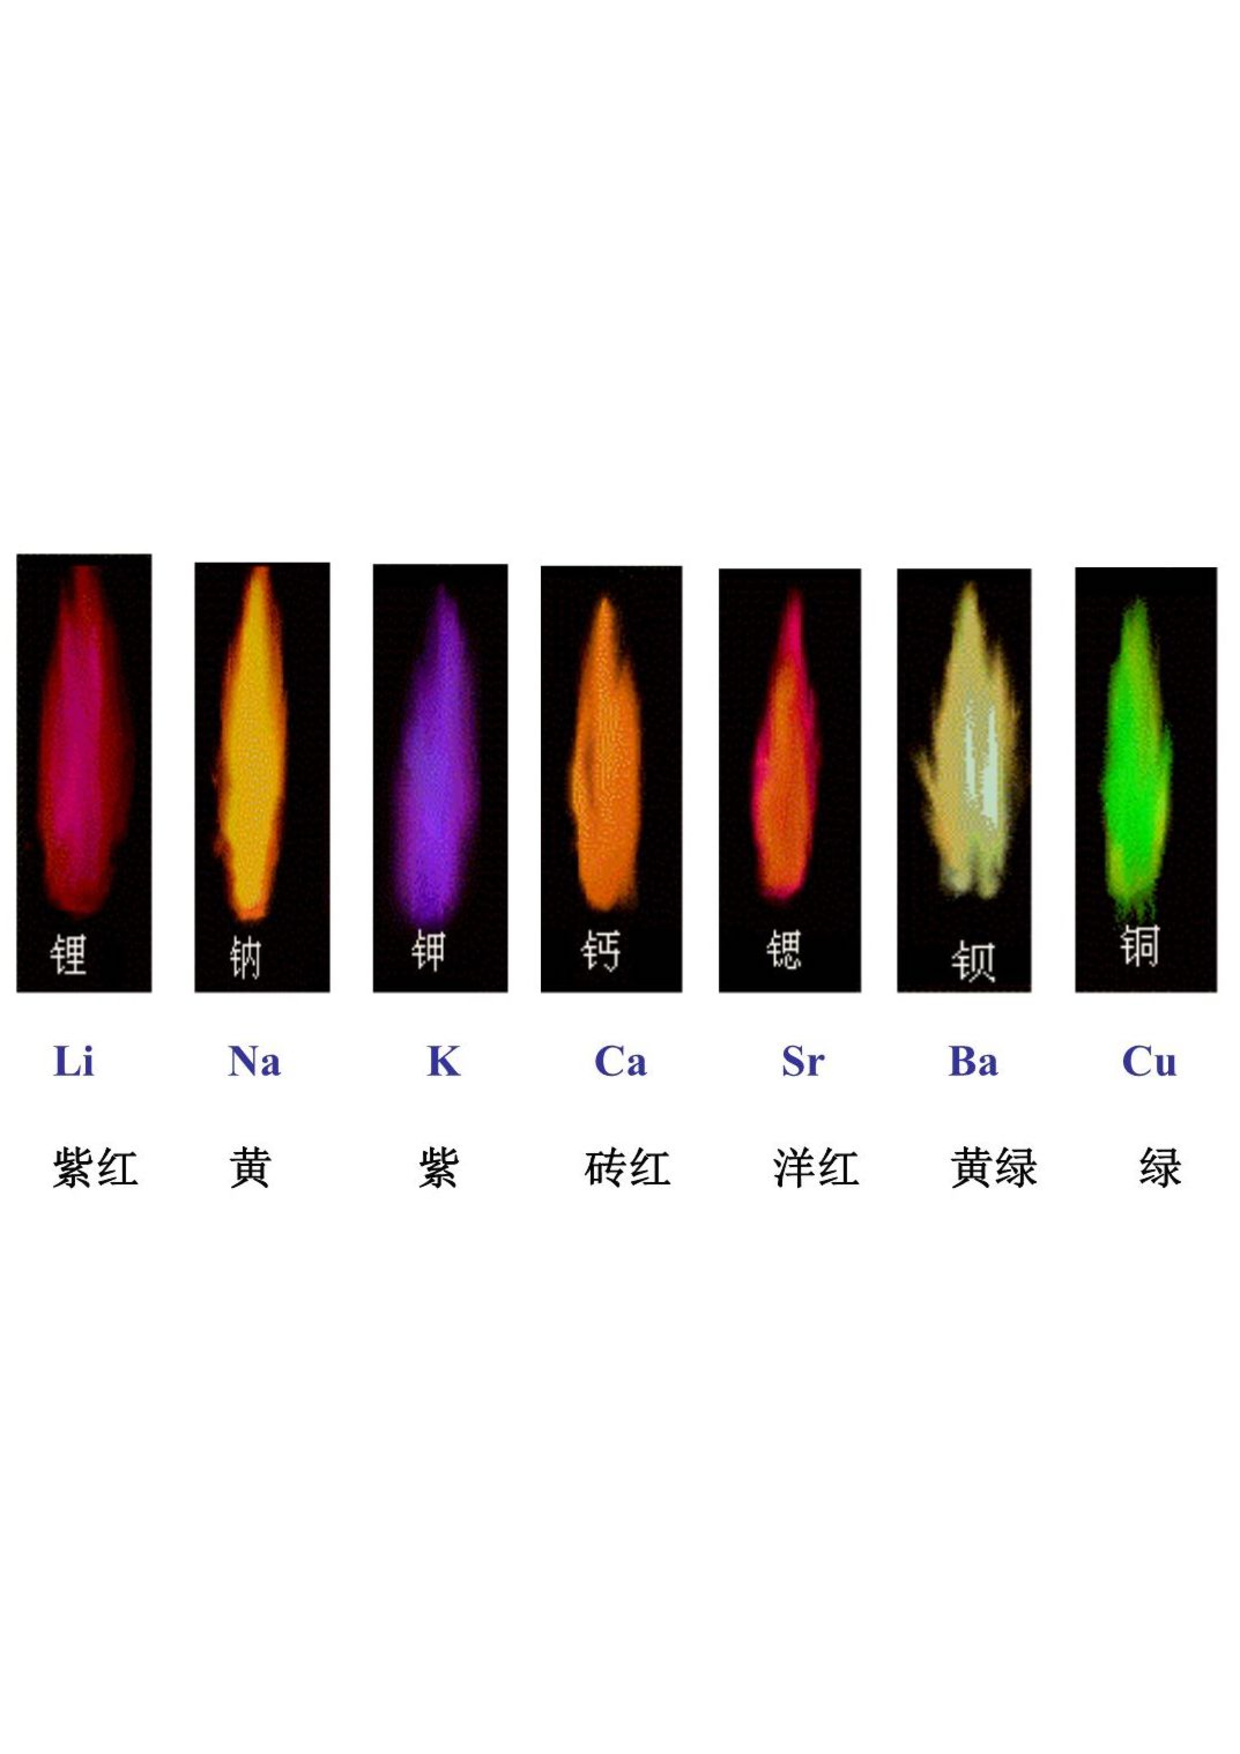
\includegraphics[scale=0.5]{res/FlameTest.pdf}
	\end{figure}
	
	
	\subsection{气体检验}
	
	\subsection{官能团检验}
	
	
	\clearpage
	\section{物质分离提纯}
	
	
	\subsection{物理法}
	
	\subsubsection{分液萃取}
	\paragraph{萃取分液条件}
	萃取物质在两种溶剂中溶解度不同,萃取剂和原溶剂不相容,萃取剂和原溶质、原溶剂均不发生反应。
	\paragraph{操作方法}
	萃取后先将下层液体从分液漏斗中放出,再将上层液体从上口放出。注意使瓶塞上的凹槽对准小孔以平衡气压。
	
	\subsubsection{过滤}
	
	\subsubsection{蒸发和结晶}
	
	\subsubsection{蒸馏}
	
	\subsubsection{升华}
	
	\subsubsection{渗析}
	
	
	\subsection{化学法}
	
	\subsubsection{沉淀法}
	\paragraph{\ce{Al2O3}和\ce{MgO}固体}
	\begin{enumerate}
		\item \ce{NaOH}溶液:过滤得\ce{Al()}和\ce{MgO}固体
		\item 稀\ce{HCl}:得氢氧化铝
		\item 加热氢氧化铝:得氧化铝
	\end{enumerate}
	\paragraph{\ce{Fe2O3}和\ce{SiO2}固体}
	\begin{enumerate}
		\item 稀\ce{HCl}:得\ce{FeCl3}溶液和\ce{SiO2}固体
		\item \ce{NaOH}溶液:得\ce{Fe(OH)3}沉淀
		\item 加热氢氧化铝:得氧化铝
	\end{enumerate}
	\paragraph{\ce{AlCl3}和\ce{FeCl3}的混合溶液}
	\begin{enumerate}
		\item \ce{NaOH}溶液:得\ce{Fe(OH)3}沉淀和\ce{AlCl3}溶液
		\item 稀\ce{HCl}:得\ce{FeCl3}溶液
	\end{enumerate}
	
	\subsubsection{氧化还原法}
	
	\subsubsection{加热分解法}
	
\end{document}